\documentclass[11pt]{report}
\linespread{1.3}
\usepackage[english]{babel}
\usepackage[utf8]{inputenc}
\usepackage{libertine}
\usepackage{libertinust1math}
\usepackage[T1]{fontenc}
\usepackage{setspace}
\usepackage{comment}
\usepackage[table,xcdraw,dvipsnames]{xcolor}
\usepackage{multirow}
\usepackage{colortbl}
\usepackage{xcolor}
\usepackage{hhline}
\usepackage{titlesec}
\usepackage{vcell}
\usepackage[export]{adjustbox} % also loads graphicx

\titleformat{\chapter}[display]
  {\Huge\bfseries}
  {}
  {0pt}
  {\thechapter.\ }

\titleformat{name=\chapter,numberless}[display]
  {\Huge\bfseries}
  {}
  {0pt}
  {}
\titlespacing*{\chapter}{0pt}{-50pt}{40pt}

\usepackage{chngcntr}
\counterwithout{figure}{chapter}

\usepackage[top=2.5cm, bottom=2.5cm, left=2cm, right=2cm]{geometry}

\usepackage{datetime}
\newdateformat{monthyeardate}{%
  \monthname[\THEMONTH], \THEYEAR}

\usepackage{subcaption}

% Math packages
\usepackage{mathtools}
\usepackage{amsfonts}
\usepackage{amssymb}
\DeclarePairedDelimiter{\ceil}{\lceil}{\rceil}

\usepackage{enumitem}
\usepackage{algorithm}
\usepackage[noend]{algpseudocode}

\algblock[Class]{Class}{EndClass}
\algblockdefx[Class]{Class}{EndClass}
    [1]{\textbf{class} \textsc{#1}}
    {\textbf{end class}}
\makeatletter
\ifthenelse{\equal{\ALG@noend}{t}}{\algtext*{EndClass}}{}
\makeatother

\algblock[Method]{Method}{EndMethod}
\algblockdefx[Method]{Method}{EndMethod}
    [2]{\textbf{method} \textsc{#1}{(#2)}}
    {\textbf{end method}}
\makeatletter
\ifthenelse{\equal{\ALG@noend}{t}}{\algtext*{EndMethod}}{}
\makeatother

\newcommand\norm[1]{\left\lVert#1\right\rVert}
\DeclareMathOperator*{\argmin}{argmin}

\usepackage{listings}
\usepackage{bera}
\usepackage{xcolor}

\lstset{language=Java,
  backgroundcolor=\color{lightgray!10!white},
  frame=tb,
  numbers=left,
  showspaces=false,
  showtabs=false,
  breaklines=true,
  showstringspaces=false,
  breakatwhitespace=true,
  commentstyle=\color{green!40!black},
  keywordstyle=\color{magenta},
  stringstyle=\color{blue},
  basicstyle=\ttfamily,
  moredelim=[is][\textcolor{grey}]{\%\%}{\%\%}
}


\colorlet{punct}{red!60!black}
\definecolor{background}{HTML}{EEEEEE}
\definecolor{delim}{RGB}{20,105,176}
\colorlet{numb}{magenta!60!black}
\definecolor{mybrown}{RGB}{152, 84, 8}
\definecolor{mygreen}{RGB}{133, 153, 0}
\definecolor{mydark}{RGB}{27, 62, 73}

\lstdefinestyle{jsonstyle}{
    basicstyle=\fontsize{14}{20}\ttfamily,
    numbers=left,
    numberstyle=\scriptsize,
    stepnumber=1,
    numbersep=8pt,
    showstringspaces=false,
    breaklines=true,
    frame=lines,
    backgroundcolor=\color{background},
    literate=
     *{0}{{{\color{numb}0}}}{1}
      {1}{{{\color{numb}1}}}{1}
      {2}{{{\color{numb}2}}}{1}
      {3}{{{\color{numb}3}}}{1}
      {4}{{{\color{numb}4}}}{1}
      {5}{{{\color{numb}5}}}{1}
      {6}{{{\color{numb}6}}}{1}
      {7}{{{\color{numb}7}}}{1}
      {8}{{{\color{numb}8}}}{1}
      {9}{{{\color{numb}9}}}{1}
      {:}{{{\color{punct}{:}}}}{1}
      {,}{{{\color{punct}{,}}}}{1}
      {\{}{{{\color{delim}{\{}}}}{1}
      {\}}{{{\color{delim}{\}}}}}{1}
      {[}{{{\color{delim}{[}}}}{1}
      {]}{{{\color{delim}{]}}}}{1},
}

\usepackage[hidelinks]{hyperref}

\begin{document}

{\setstretch{1.0}
  \begin{titlepage}
  	\centering
  	{\huge UNIVERSITY OF PISA\par}
  	\vspace{1cm}
  	\includegraphics[width=5cm]{img/cherubino.png}\par
  	\vspace{1cm}
  	{\LARGE School of Engineering \par}
  	\vspace{0.5cm}
  	{\LARGE Master of Science in Computer Engineering\par}
  	\vspace{0.5cm}
  	{\LARGE Large Scale And Multi-Structured Databases\par}
  	\vspace{1.5cm}
  	{\large PROJECT DOCUMENTATION\par}
  	{\LARGE \textbf{PSEUDOSTACKOVERFLOW: A JAVA + MONGODB + NEO4J BASED APPLICATION IMPLEMENTING A SIMPLE PROGRAMMING FORUM}\par}
  	\vspace{2.5cm}
  	\begin{flushleft}
  	\large{WORKGROUP:\par}
  	\vspace{0.2cm}
  	\large{Leandro Giacomazzo\par}
  	\vspace{0.2cm}
  	\large{Iacopo Pacini\par}
  	\vspace{0.2cm}
  	\large{Gaetano Niccolò Terranova\par}
  	\end{flushleft}
  	\vfill

    % Bottom of the page
  	{\large ACADEMIC YEAR 2021/2022\par}
  \end{titlepage}
}

\pagenumbering{arabic}
\addtocounter{page}{1}

\tableofcontents

\newpage

\chapter{Introduction}\label{introduction}
PseudoStackOver is a programming forum in which professional  programmers or simply enthusiasts can publish programming/IT related questions. All questions are public, everyone can browse them but only registered users can answer and mark with positive or negative vote already existing answers. Every user is equipped with a personal profile containing a brief description uploaded by the user, her location and a profile picture. Users can "follow" each other and periodically check if one of their follower posts new questions or simply answers to a post.
The complete code can be found at this address:
\url{https://github.com/gaetanoterra/progettoLSMD}

\section{Functional Requirements}
This section  shows the main functional requirements of the application:
\begin{itemize}
  \item The platform allows to be navigated in three types of modes: unregistered mode, register mode, admin mode.
  \item Any user should be able to browse the stored posts
  \item A registered user should be able to remove a post of his own
  \item A registered user should be able to remove an answer of his own
  \item A registered user should be able to answer any stored post
  \item A registered user should be able to vote an already existing answer
  \item A registered user should be able to browse his followed users list
  \item A registered user should be able to Enter and update their personal information
  
\end{itemize}
\newpage
\section{Non-Functional Requirements}
This section shows the main non-functional requirements of the application:
\begin{itemize}
  \item The application must have a low response time.
  \item The application must guarantee data availability.
  \item The application must ensure prevention against server crashes thanks to replicas.
  \item Admins of the application periodically monitor the behaviour of Users in order to guarantee that they comply to the Terms \& Agreements.
  
\end{itemize}
\chapter{Design} \label{design}
\section{UML Use Cases Diagram}
    \includegraphics[width=\textwidth,keepaspectratio=true]{img/use_cases.png}\par

\newpage

\section{UML Analysis Class Diagram}
    \includegraphics[width=\textwidth,keepaspectratio=true]{img/class-diagram.png}\par
\newpage


\chapter{Implementation}\label{implementation}

\section{Document Database}

The document part of the application is implemented using MongoDB, a source-available cross-platform document-oriented database program. Classified as a NoSQL database program, MongoDB uses JSON-like documents with optional schemas. The document database contains two collections: Users and Posts listed below.
\newline

\begin{lstlisting}[
    style = jsonstyle,
    title=\textbf{Posts document structure},
    frame=tlrb,
    xleftmargin=0.2\textwidth,
    xrightmargin=0.2\textwidth
]
{
    _id: ObjectId,
    AnswerId: string,
    CreationDate: long,
    ViewCount: int,
    Body: string,
    Title: string,
    Tags: [ string ],
    DisplayName: string,
    Answers:
        [{
            Id: string,
            CreationDate: long,
            Body: String,
            OwnerDisplayName: string,
            Score: int
        }]
}
\end{lstlisting}

\newpage

The latter document contains all the information related to a question posted on the forum, in particular:
\begin{itemize}
  \item \textbf{GlobalId} computed as \\ 
  \centerline {\textbf{SHA256(\{ Title | CreationDate \})}} \\
  It allows to identify univoquely a post among the two databases.
  \item \textbf{CreationDate} is a long value representing the date and the time in which that particular question is uploaded into the forum;
  \item \textbf{ViewCount} field keeps track of the overall times in which that post is read;
  \item \textbf{Body} contains the actual question, namely its text body;
  \item \textbf{Title} contains the title of the question;
  \item \textbf{Tags} is a list of tag names that the a user encloses to the post itself;
  \item \textbf{DisplayName} is the username of the author;
  \item \textbf{Answers} is a list of documents containing creation date, text body, author username and the algebraic sum of the received votes. The choice of embedding this collection is due to the fact that the answers to a post are generally limited to a few units. Moreover, this setting allows to populate entirely the FullPostInterface(one of the most requested) with a single find() query on \_id field.
\end{itemize}

\begin{lstlisting}[
    style = jsonstyle,
    title={Users document structure},
    frame=tlrb,
    xleftmargin=0.5\linewidth
]
{
    _id: ObjectId,
    Reputation: int,
    CreationDate: long,
    DisplayName: string,
    WebsiteUrl: string,
    Location: string,
    AboutMe: string,
    ProfileImageUrl: string,
    Password: string,
    followerNumber: int,
    followedNumber: int,
    IsAdmin: boolean
}
\end{lstlisting}

\begin{itemize}
  \item \textbf{Reputation} The algebraic sum of the Votes given to the answers given by the user itself;
  \item \textbf{CreationDate} is a long value representing the date and the time in which that particular user joined the forum;
  \item \textbf{DisplayName} is the username of the user;
  \item \textbf{WebSiteUrl} user personal web-site URL;
  \item \textbf{Location} where the user is located;
  \item \textbf{AboutMe} contains the title of the question;
  \item \textbf{ProfileImageUrl} is a list of tag names that the a user encloses to the post itself;
  \item \textbf{Password} User profile password;
  \item \textbf{followerNumber} Amount of user following that particular profile;
  \item \textbf{followedNumber} Amount of user followed by that particular user;
  \item \textbf{isAdmin} optional field indicating that the user has administrator priviledges;
\end{itemize}

\newpage

\subsection{Queries Analysis}
    \begin{table}[h]
    \centering

    \begin{tabular}{|p{0.20\linewidth}p{0.20\linewidth}m{0.20\linewidth}|}
        \hline
        \rowcolor[HTML]{9B9B9B} 
        \multicolumn{3}{|c|}{\cellcolor[HTML]{9B9B9B}\textbf{Read Operations}} 
        \\ \hline
        \rowcolor[HTML]{EFEFEF} 
        \multicolumn{1}{|c|}{\cellcolor[HTML]{EFEFEF}Operation}                                                                                                             & \multicolumn{1}{c|}{\cellcolor[HTML]{EFEFEF}\begin{tabular}[c]{@{}c@{}}Expected\\ Frequency\end{tabular}} & Cost                 \\ \hline
        \rowcolor[HTML]{FFFFFF} 
        \multicolumn{1}{|c|}{\cellcolor[HTML]{FFFFFF}\begin{tabular}[c]{@{}c@{}}Retrieve complete informations\\ about a post by Post title/body\end{tabular}}              & \multicolumn{1}{c|}{\cellcolor[HTML]{FFFFFF}\begin{tabular}[c]{@{}c@{}}Very\\ High\end{tabular}}          & Medium\newline(text search) \\ \hline
        \rowcolor[HTML]{FFFFFF} 
        \multicolumn{1}{|c|}{\cellcolor[HTML]{FFFFFF}\begin{tabular}[c]{@{}c@{}}Retrieve complete informations\\ about a post by Post title/body\end{tabular}}              & \multicolumn{1}{c|}{\cellcolor[HTML]{FFFFFF}\begin{tabular}[c]{@{}c@{}}Very\\ High\end{tabular}}          & Low\newline(search by \_id)  \\ \hline
        \rowcolor[HTML]{FFFFFF} 
        \multicolumn{1}{|c|}{\cellcolor[HTML]{FFFFFF}\begin{tabular}[c]{@{}c@{}}Retrieve complete informations about a User\\ given his(her) username\end{tabular}}         & \multicolumn{1}{c|}{\cellcolor[HTML]{FFFFFF}High}                                                         & Medium\newline(text search) \\ \hline
        \rowcolor[HTML]{FFFFFF} 
        \multicolumn{1}{|c|}{\cellcolor[HTML]{FFFFFF}\begin{tabular}[c]{@{}c@{}}Given a tag, find the users who answers gained the highest \\score with their answers. \end{tabular}} & \multicolumn{1}{c|}{\cellcolor[HTML]{FFFFFF}Low}                                                          & High\newline(aggregation)    \\ \hline
    \end{tabular}
\end{table}

\begin{table}[h]
    \centering 
    \begin{tabular}{|p{0.33\linewidth}p{0.33\linewidth}p{0.33\linewidth}|}
        \hline
        \rowcolor[HTML]{9B9B9B} 
        \multicolumn{3}{|c|}{\cellcolor[HTML]{9B9B9B}\textbf{Write Operations}}                                                                                                                                                                                                   \\ \hline
        \rowcolor[HTML]{EFEFEF} 
        \multicolumn{1}{|c|}{\cellcolor[HTML]{EFEFEF}Operation}                                                                       & \multicolumn{1}{c|}{\cellcolor[HTML]{EFEFEF}\begin{tabular}[c]{@{}c@{}}Expected\\ Frequency\end{tabular}} & Cost                          \\ \hline
        \rowcolor[HTML]{FFFFFF} 
        \multicolumn{1}{|c|}{\cellcolor[HTML]{FFFFFF}\begin{tabular}[c]{@{}c@{}}Insert/remove a new Answer/Post/User\end{tabular}} & \multicolumn{1}{c|}{\cellcolor[HTML]{FFFFFF}Low}                                                         & Average (document add/remove) \\ \hline
        \rowcolor[HTML]{FFFFFF} 
        \multicolumn{1}{|c|}{\cellcolor[HTML]{FFFFFF}\begin{tabular}[c]{@{}c@{}}Update Answer\\ Score\end{tabular}}                   & \multicolumn{1}{c|}{\cellcolor[HTML]{FFFFFF}Average}                                                         & Low (1 attribute write)       \\ \hline
        \rowcolor[HTML]{FFFFFF} 
        \multicolumn{1}{|c|}{\cellcolor[HTML]{FFFFFF}Update user data}                                                                & \multicolumn{1}{c|}{\cellcolor[HTML]{FFFFFF} Very Low}                                                          & Low (few attributes write)    \\ \hline
        \end{tabular}
\end{table}

All the assumption made previously are based on the fact that a question(or an answer) is posted only once and accessed many times by both registered and anonymous users, the same holds for Users data. It can be concluded that the queries are predominantly read intensive, for this reason indexes to speed up read operations (at the expense of write operations) are added.

\newpage
\subsection{Queries Implementation}



\begin{table}[H]
\centering
\begin{tabular}{|m{11cm}|m{5cm}|} 
\hline
\rowcolor[rgb]{0.937,0.937,0.937} \multicolumn{1}{|c|}{\textbf{Query}} & \multicolumn{1}{c|}{\textbf{Description}} \\ 
\hline
\textcolor{mydark}{db.Posts.aggregate(}
    \par
    ~~\textcolor{mydark}{[}\par
    ~~~~ \textcolor{mydark}{\{}\textcolor{mybrown}{\$match}: \textcolor{mydark}{\{}\textcolor{mygreen}{"Tags":"??"}\textcolor{mydark}{\}}\textcolor{mydark}{\}},\par
    ~~~~~~\textcolor{mydark}{\{}\textcolor{mybrown}{\$unwind}: \textcolor{mygreen}{"\$Answers"}\textcolor{mydark}{\}},\par
    ~~~~~~\textcolor{mydark}{\{}\textcolor{mybrown}{\$match}: \textcolor{mydark}{\{}\textcolor{mygreen}{"Answers.DisplayName"}:\textcolor{mydark}{\{}\textcolor{mybrown}{\$ne}:\textcolor{red}{null}\textcolor{mydark}{\}}\textcolor{mydark}{\}}\textcolor{mydark}{\}},\par
    ~~~~~~\textcolor{mydark}{\{}\textcolor{mybrown}{\$group}: \par
    ~~~~~~\textcolor{mydark}{\{}\par
    ~~~~~~~~\textcolor{mydark}{\_id:} \textcolor{mygreen}{"\$Answers.DisplayName"},\par
    ~~~~~~~~\textcolor{mydark}{totaleRisposteUtente:\{}\textcolor{mybrown}{\$sum}:\textcolor{mygreen}{"\$Answers.Score"}\textcolor{mydark}{\}}\textcolor{mydark}{\}}\par
    ~~~~~~\textcolor{mydark}{\},}\par
    ~~~~~~~\textcolor{mydark}{\{}\textcolor{mybrown}{\$sort}: \textcolor{mydark}{\{}\textcolor{mygreen}{ "totaleRisposteUtente"}: -1 \textcolor{mydark}{\}} \textcolor{mydark}{\}}\par
    ~~~~\textcolor{mydark}{]}\par
\textcolor{mydark}{)} & This query allows to retrieve 
the most expert users on a given tag. Namely the ones whose answers gained he highest score\\ 
\hline
\textcolor{mydark}{db.Posts.find(}\par
~~~~\textcolor{mydark}{\{}\par
~~~~~~~~\textcolor{mybrown}{\$text}\textcolor{mydark}{:\{}\textcolor{mybrown}{\$search}: \textcolor{mygreen}{"??"}\textcolor{mydark}{\},}\par
~~~~~~~~\textcolor{mybrown}{\$or}\textcolor{mydark}{:[}\par
~~~~~~~~~~~~\textcolor{mydark}{\{Title: \{}\textcolor{mybrown}{\$regex}: \textcolor{mygreen}{/.*??.* /i}\textcolor{mydark}{\}\},}\par
~~~~~~~~~~~~\textcolor{mydark}{\{Body:\{}\textcolor{mybrown}{\$regex}: \textcolor{mygreen}{/.*??.* /i}\textcolor{mydark}{\}\}}\par
~~~~~~~~\textcolor{mydark}{]}\par
~~~~\textcolor{mydark}{\},}\par
~~~~\textcolor{mydark}{\{}\par
~~~~~~\textcolor{mydark}{\_id:}\textcolor{mygreen}{ 1}\textcolor{mydark}{,}\par
~~~~~~\textcolor{mydark}{Title:}\textcolor{mygreen}{ 1}\textcolor{mydark}{,}\par
~~~~~~\textcolor{mydark}{Tags:}\textcolor{mygreen}{ 1}\textcolor{mydark}{,}\par
~~~~~~\textcolor{mydark}{numberOfAnswers:\{}\textcolor{mybrown}{\$size}:\textcolor{mygreen}{"\$Answers" }\textcolor{mydark}{\},}\par
~~~~~~\textcolor{mydark}{ViewCount:}\textcolor{mygreen}{ 1}\textcolor{mydark}{,}\par
~~~~\textcolor{mydark}{\},}\par
\textcolor{mydark}{);}
 & This query is a crucial feature for the forum, it is one of the most used, it can be exploited by both registered andanonymus users.  \\
\hline
\textcolor{mydark}{db.Users.find(\{}\textcolor{mybrown}{DisplayName}\textcolor{mydark}{:} \textcolor{mygreen}{"??"}\textcolor{mydark}{\})}
 & It allows to retrieve all the question asked by a user,
it exploits an index on the username.  \\
\hline
\end{tabular}
\end{table}
The most critical operations, as previously stated, are the log-in operation and the search by text. For this reason it has been chosen to create a compound text index on the fields Title and Body in the Posts collection and a text index in the displayName field in the Users collection.
The compound index in all the benchmarks boosted the query performance at least of a factor ten. The index on the Users collection instead caused an even greater speed-up of two orders of magnitude in all benchmarks.
\newpage
\section{Graph Database}
    
    \begin{center}
        \includegraphics[
            width=0.8\textwidth,
            keepaspectratio=true
        ]{img/neo4j_draft.png}
        \par
    \end{center}

    
    \subsection{Nodes}
        \begin{itemize}
            \item \textbf{User}, representing the users registered within the application, having as attribute its own username
            \item \textbf{Question}, representing a question asked by a user with its global id and its title. The question body is kept in the document db.
            \item \textbf{Answer}, representing an answer given to a particular question
            \item \textbf{Tag}, An unambiguous container for a particular tag.
        \end{itemize}
    \newpage
    \subsection{Relationships}
        \begin{itemize}
            \item \textbf{User $\rightarrow$ ANSWERS\_WITH $\rightarrow$ Answer} which connects an answer with its own author.
            This relationship has no attributes.
            \item \textbf{Answer$\rightarrow$ BELONGS\_TO $\rightarrow$ Question}, which connects a question with its own author.
            This relationship has no attributes.
            \item \textbf{Question$\rightarrow$ CONTAINS\_TAG $\rightarrow$ Tag}, which connects a question with the corresponding tag Entity. This relationship has no attributes.
            \item \textbf{User $\rightarrow$ FOLLOW $\rightarrow$ User},  which represents a user
            following another in the application, and is
            created/removed when a User adds/removes another
            User from his followed users list.
            This relationship has no attributes.
            \item \textbf{User $\rightarrow$ POSTS\_QUESTION $\rightarrow$ Question} which represents a user
            uploading a question on the forum, and is created/removed when a User posts/removes a question. This relationship has no attributes.
            \item \textbf{User $\rightarrow$ VOTE $\rightarrow$ Answer}, which represents a user adding a positive or negative vote to an answer.
            It contains an integer +1 or -1 representing a positive/negative vote as attribute.
        \end{itemize}
    \newpage   
    \subsection{Queries Analysis} 
     \begin{table}[h]
    \centering
    \begin{tabular}{|c|c|c|} 
    \hline
    \multicolumn{3}{|c|}{{\cellcolor[rgb]{0.608,0.608,0.608}}\textbf{Read Operations}}                                                                                                                                                                                                                                                 \\ 
    \hline
    \rowcolor[rgb]{0.937,0.937,0.937} Operation                                                                                               & \begin{tabular}[c]{@{}>{\cellcolor[rgb]{0.937,0.937,0.937}}c@{}}Expected\\ Frequency\end{tabular} & Cost                                                                               \\ 
    \hline
    \begin{tabular}[c]{@{}c@{}}Retrieve answers posted by a given user along with the~\\total score\end{tabular}                              & Low                                                                                               & \begin{tabular}[c]{@{}c@{}}Medium\\(multiple reads and\\adjacencies)\end{tabular}  \\ 
    \hline
    \begin{tabular}[c]{@{}c@{}}Retrieve users who post questions containing\\the same tag of the questions asked given by a given user\end{tabular}                                       & Average                                                                                           & \begin{tabular}[c]{@{}c@{}}Medium\\(multiple reads and\\adjacencies)\end{tabular}  \\ 
    \hline
    retrieve the follower list of a given user                                                                                                & High                                                                                              & Low                                                                                \\ 
    \hline
    retrieve the list of users followed by a certain user                                                                                     & High                                                                                               & Low                                                                                \\ 
    \hline

    \begin{tabular}[c]{@{}c@{}}Retrieve the topics(in terms of tags) that \\sparked interests among the most followed users.\end{tabular}     & Low                                                                                               & High                                                                               \\ 
    \hline
    \begin{tabular}[c]{@{}c@{}}retrieve the questions asked by the most followed users\\~who have the highest number of answers\end{tabular} & Low                                                                                               & High                                                                               \\
    \hline
    \end{tabular}
\end{table}

\begin{table}[h]
\centering
\begin{tabular}{|c|c|l|} 
\hline
\multicolumn{3}{|c|}{{\cellcolor[rgb]{0.608,0.608,0.608}}\textbf{Write Operations}}                                                                     \\ 
\hline
\rowcolor[rgb]{0.937,0.937,0.937} Operation & \begin{tabular}[c]{@{}>{\cellcolor[rgb]{0.937,0.937,0.937}}c@{}}Expected\\ Frequency\end{tabular} & Cost  \\ 
\hline
Insert/remove a new Question/Post/Answer    & Low                                                                                               & Low   \\ 
\hline
Insert a Vote relation                       & Average                                                                                           & Low   \\
\hline
\end{tabular}
\end{table}
    
    \newpage
    \subsection{Queries Implementation}
    \begin{table}[H]
        \centering
        \begin{tabular}{|m{13cm}|m{5cm}|} 
        \hline
        \rowcolor[rgb]{0.937,0.937,0.937} \multicolumn{1}{|c|}{\textbf{Query}} & \multicolumn{1}{c|}{\textbf{Description}} \\ 
        \hline
        \textcolor{mygreen}{MATCH} (topUsers:User)<-[f:FOLLOW]-(otherUsers:User)\par
\textcolor{mygreen}{WITH} topUsers\.displayName \textcolor{mygreen}{as} t\_us, count(\*) \textcolor{mygreen}{as} follower\_no\par
\textcolor{mygreen}{ORDER BY} follower\_no
\textcolor{mygreen}{DESC LIMIT} 10 \par
\textcolor{mygreen}{MATCH} (t:Tag)<-[c\_tag:CONTAINS\_TAG]-(q:Question)\par
~~~~~~~~~~~~~~<-[b\_to:BELONGS\_TO]-(a:Answer)\par
~~~~~~~~~~~~~~<-[an\_with:ANSWERS\_WITH]-(u:User{displayName:t\_us})\par
\textcolor{mygreen}{WITH} u.displayName \textcolor{mygreen}{as} top\_users,\par
~~~~~~~~~~follower\_no,\par
~~~~~~~~~~t.tagNames \textcolor{mygreen}{as} tag\_names,\par
~~~~~~~~~~count(\*) \textcolor{mygreen}{as} tags\_top\_users \par
\textcolor{mygreen}{ORDER BY} tags\_top\_users  \textcolor{mygreen}{DESC} \par
\textcolor{mygreen}{RETURN} top\_users, follower\_no, tag\_names, tags\_top\_users \par
\textcolor{mygreen}{LIMIT} 10 & This query retrieves the questions asked by the most followed users \par who have the highest number of answers \\ 
        \hline
        \textcolor{mygreen}{MATCH} (topUsers:User)<-[f:FOLLOW]-(otherUsers:User)\par
\textcolor{mygreen}{WITH} topUsers.displayName \textcolor{mygreen}{as} top\_users, \textcolor{mygreen}{count}(\*) as folllower\_no\par
\textcolor{mygreen}{ORDER BY} folllower\_no DESC LIMIT 10\par
\textcolor{mygreen}{CALL} \{\par
    ~~~~~~\textcolor{mygreen}{WITH} top\_users \par
    ~~~~~~\textcolor{mygreen}{MATCH} (a:Answer)-[b\_to:BELONGS\_TO]->(quest:Question)\par
    ~~~~~~~~~~~~<-[pq:POSTS\_QUESTION]-(u:User{displayName:top\_users})\par
    ~~~~~~\textcolor{mygreen}{WITH} u.displayName \textcolor{mygreen}{as} t\_users,\par
    ~~~~~~~~~~~~~~~~quest.Title \textcolor{mygreen}{as} title, \par
    ~~~~~~~~~~~~~~~~\textcolor{mygreen}{count}(\*) \textcolor{mygreen}{as} answers\_no\par
    ~~~~~~\textcolor{mygreen}{ORDER BY} u.displayName, answers\_no \textcolor{mygreen}{DESC}\par
    ~~~~~~\textcolor{mygreen}{LIMIT} 3\par
    ~~~~~~\textcolor{mygreen}{RETURN} title, answers\_no\par
\}\par
\textcolor{mygreen}{RETURN} top\_users, title, answers\_no          & Retrieve the topics(in terms of tags) that \par sparked interests among the most followed users.    \\ 
        \hline
         db.\textcolor{mygreen}{index}.fulltext.queryNodes(\textcolor{Dandelion}{"displayname\_fulltext\_index"}, \textcolor{Dandelion}{"???"})\par
\textcolor{mygreen}{YIELD node}\par
\textcolor{mygreen}{MATCH} (node)-[:ANSWERS\_WITH]->(a:Answer)\par
~~~~~~~~~~~~<-[v:VOTE]-(uv:User)\par
\textcolor{mygreen}{RETURN} a.answerId as answerId,\par
~~~~~~a.body as body, \par
~~~~~~sum(v.VoteTypeId) as score \par
\textcolor{mygreen}{ORDER BY} score \textcolor{mygreen}{DESC}

  & Retrieve answers posted by a given user along with the \par total score  \\ 
        \hline
       
        \end{tabular}
    \end{table}
    
\newpage

\begin{table}
    \centering
    \begin{tabular}{|m{13cm}|m{5cm}|} 
    \hline
    \textcolor{mygreen}{MATCH}  (u2: User)-[:POSTS\_QUESTION]->(:Question)\par 
-[:CONTAINS\_TAG]->(t:Tag {tagNames: \textcolor{Dandelion}{"???"} })\par
WHERE u2.displayName <> \textcolor{Dandelion}{"???"}  \par
\textcolor{mygreen}{RETURN distinct}  u2.displayName \textcolor{mygreen}{AS}  Username, \par
~~~~~~~~~~~~~~~~u2.profileImage \textcolor{mygreen}{AS}  profileImage \par
\textcolor{mygreen}{LIMIT}  10; & Retrieve users who post questions containing the same tag of the questions asked given by a given user   \\
    \hline
    \textcolor{mygreen}{MATCH}  (u3:User)<-[:FOLLOW]-(u2:User)\par
~~~~~~~~~~~~~~<-[:FOLLOW]-(u:User displayName: \textcolor{Dandelion}{"???"})\par
\textcolor{mygreen}{WHERE}  u3 <> u \textcolor{mygreen}{and}  u3 <> u2 \par
\textcolor{mygreen}{RETURN distinct}  u3.displayName  \textcolor{mygreen}{AS}  Username, \par
~~~~~~~~~~~~~~~u3.profileImage \textcolor{mygreen}{AS}  profileImage \par
\textcolor{mygreen}{LIMIT}  20; & Given a user Retrieve a list of "friends of friends", namely people that the user does not follow by are followed by the people the user itself is following   \\
    \hline
    \end{tabular}
\end{table}
As depicted in the above tables, most queries requires the displayName of the user. In order to avoid that this parameter could be a bottleneck became a bottleneck for the entire graph a FULL\_TEXT index has been added to the db. The Benchmarks show that such index could increase the search performance every time, at least, of a factor of 10.
\newpage

\section{Cross\-Database Coherence}
In our application there are some operations, like insert a new User or eliminate a Post, that have to access to both Document and Graph databases. Of course we want that if an operation is performed on the first one, it would be performed also in the other one. To do this we created an \textbf{\emph{error.log}} file where possible errors during an operation are stored. Specifically the operations Insert/Remove User, Insert/Remove Post, Insert/Remove Answer and Insert/Remove Vote need to check if the operation is correctly performed on the first database, if it is not an error is appended into the file. On the follow a schema of the process is shown; for brevity, we show just two examples because the procedure is the same for all cases.

\begin{figure}[ht]
  \centering
  \includegraphics[width=\textwidth,keepaspectratio=true]{img/Consistency.jpg}
  \caption{Cross-Database Coherence for an Insert/Remove operation}
\end{figure}

\newpage

\section{Cluster topology}
The database cluster on which the server relies consists of 3 servers (available on the UNIPI network). An instance of MongoDB was deployed on every server (joined together in a replica set), meanwhile Neo4j was deployed on only one server, due to it being the Community Edition (thus not allowing the whole core/replica architecture).

\begin{figure}[ht]
  \centering
  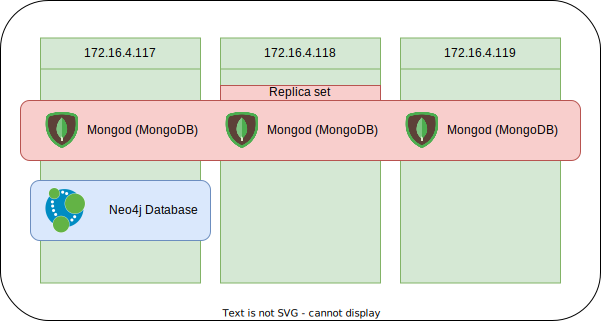
\includegraphics[width=\textwidth,keepaspectratio=true]{img/cluster_diagram.png}
  \caption{Cluster diagram}
\end{figure}
A further improvement on the availability could be achieved by deploying the document database on a sharded architecture. A possible sharding key capable of distribute in a relatively could be the \_id field inserted by the DMBS itself. This field, in fact, is computed by means of an hash algorithm on the document itself. Hash algorithms are able per design to produce random values uniformly distributed on a quite wide spectrum of values(given by the digest length itself). 
\newpage
 
\section{Server Package}
The Server package contains a total number of seven Java classes; these classes are in charge to run the server, to handle the requests coming from the clients and to communicate with both document and graph databases. on the follow these classes are described more in detail.

\begin{figure}[H]
  \centering
  \includegraphics[
    width=\textwidth,
    max height=19cm,
    keepaspectratio=true
    ]{img/packages/Package_server.png}
  \caption{server package UML diagram}
\end{figure}

\subsection{Server}
The server class contains a constructor which take three arguments: the \textit{port number} where the server listen for a client connection, the \textit{backlog length} and the \textit{execution mode} of databases, meaning local or cluster mode. The \textit{waitForConnection} method is used to listen and accept a new connection with a client. Everytime a new connection is accepted, a new \textit{ClientManager} instance is created to handle messages from the connected client.

\subsection{ServerStart}
This class contains the \textit{main} method, so it is the class that actually run the server. In the main method we create a Server object and we wait for the connection with clients.
\subsection{ClientManager}
This class is instantiated when a new connection is created between server and client. This class handle the messages coming from the client: specifically a send and receive methods are used to send sand back and receive messages; these messages are then opened and forwarded to right query to be executed. The results of query are then sent back to the client.
\subsection{DBExecutionMode}
This class is a simple enumaration class to specify the methodology of databases execution between local and cluster.
\subsection{DBManager}
This class is supposed to communicate with the \textit{ClientManager}, receiving the request to be forwarded to the databases, and on the other side with Graph and Document databases. So the DBManager forward to the right database (or to both of them) driver the client request. The constructor of this class create an instance of both Graph and Document database drivers.
\subsection{DocumentDBManager}
This class is the Java driver class to make queryes to the Document database, specifically to MongoDB. The \textit{DBManager} forward the client requests to this class calling the method to run the right query. Results are then sent back to the \textit{DBManager}. The constructor of this class take as parameter the execution mode, to run in local or into a cluster; moreover is opened the connection with the database, selecting the database and the collections needed.
\subsubsection{GraphDBManager}
This class is the Java driver class to make queries to the Graph database, specifically to Neo4j. The \textit{DBManager} forward the client requests to this class calling the method to run the right query. Results are then sent back to the \textit{DBManager}. The constructor of this class take as parameter the execution mode, to run in local or into a cluster; moreover is opened the connection with the database giving database name and password.

\section{Messages}
The \textit{Messages} package contains the serializable classes used by the \textit{ServerConnectionManager} and \textit{ClientManager} to send respectively requests to the server and send back results; the objects to be sent are these messages. We created one abstract serializable class, \textit{Message}, from which we extended all other classes; moreover we added two more abstract classes to better distinguish the tasks of the extended messages. The package contains also some enumeration classes. On the follow are described in detail all messages we created.
\begin{figure}[H]
  \centering
  \includegraphics[width=\textwidth,max height=30cm,keepaspectratio=true]{img/packages/Package_Messages.png}
  \caption{messages package UML diagram}
\end{figure}
\subsection{Message}
This is an abstract class and the serializable class, from which all other Message classes are extended. This class implements the method \textit{getOpcode}, which return the Opcode, meaning the code to describe the message used by the \textit{ServerConnectionManager} and the \textit{ClientManager} to forward correctly the message.
\subsubsection{MessageLogin}
This message extends the \textit{Message} abstract class and is used to send a login request to the server, sending the User data, specifically username and password.
\subsubsection{MessageLogOut}
This message extends the \textit{Message} abstract class and is used the logout from the application, sending the username of the logged user to the server.
\subsubsection{MessageSignUp}
This message extends the \textit{Message} abstract class and is used to perform the registration of an unregistered user. Specifically into this message all data inserted by the user in the registration form are sent to the server.
\newpage
\subsection{MessageCreateDelete}
This is an abstract class, extended from the \textit{Message} class. All messages which extends this class are messages used to send a create or delete request to the server. This message implements the \textit{getOperation} method, which return the Operation to be performed (create, delete, check), and a \textit{getObject} method, to get the sent object.
\subsubsection{MessagePost}
This message extends the \textit{MessageCreateDelete} abstract class and is used to send a creation/delete request of an User to the Server.
\subsubsection{MessageUser}
This message extends the \textit{MessageCreateDelete} abstract class and is used to send a creation/delete request of a Post to the Server.
\subsubsection{MessageAnswer}
This message extends the \textit{MessageCreateDelete} abstract class and is used to send a creation/delete request of an Answer to the Server.
\subsubsection{MessageFollow}
This message extends the \textit{MessageCreateDelete} abstract class and is used to send a creation/delete/check request of a Follow relationship to the Server.
\subsubsection{MessageVote}
This message extends the \textit{MessageCreateDelete} abstract class and is used to send a creation/delete request of a Vote relationship to the Server. 
\newpage
\subsection{MessageReadObjectQuery}
This is an abstract class, extended from the \textit{Message} class. All messages which extends this class are messages used to get some content from the Server, such as User data or Posts list.This class implements the \textit{getObject} method, used to get the objects sent to and from the Server.
\subsubsection{MessageGetAnswers}
This message extends the \textit{MessageReadObjectQuery} abstract class and is used to send a request to the server to get all the Answers of the specified User.
\subsubsection{MessageGetPostsByParameter}
This message extends the \textit{MessageReadObjectQuery} abstract class and is used to send a request to the server to get a list of Posts given a specific \textit{Parameter}, chosen between Username, Id and Text.
\subsubsection{MessageGetUserData}
This message extends the \textit{MessageReadObjectQuery} abstract class and is used to send a request to the server to get all the data of a specific User. To get these data the username of the User is given.
\subsubsection{MessageGetPostData}
This message extends the \textit{MessageReadObjectQuery} abstract class and is used to send a request to the server to get all the data of a specific Post. To get these data the ID of the Post is given.
\subsubsection{MessageGetCorrelatedUsers}
This message extends the \textit{MessageReadObjectQuery} abstract class and is used to send a request to the server to get data of a list of Users given a specific username. Specifically the class contains an ArrayList of Users to contain the response of the Server.
\subsubsection{MessageGetRecommendedUsers}
This message extends the \textit{MessageReadObjectQuery} abstract class and is used to send a request to the server to get data of a list of Users given a specific tag. Specifically the class contains an ArrayList of Users to contain the response of the Server.
\subsubsection{MessageGetExpertsByTag}
This message extends the \textit{MessageReadObjectQuery} abstract class and is used to send a request to the server to get data of a list of Users. Specifically the class contains an Array of Users to contain the response of the Server and a tag String as parameter of the query.
\newpage
\subsubsection{MessageGetFollowData}
This message extends the \textit{MessageReadObjectQuery} abstract class and is used to send a request to the server to get data of a list of Users, the followers or the Followed of a specific user. Specifically the class contains an ArrayList of Users to contain the response of the Server and a tag String as parameter of the query, an username String as parameter for the query and a Boolean to choose between Follower or Followed.
\subsubsection{MessageGetTopUsersPosts}
This message extends the \textit{MessageReadObjectQuery} abstract class and is used to send a request to the server to get data of a list of Users and relative Posts. Specifically the class contains a Map of Users and Posts to store the Server response.
\subsubsection{MessageAnalyticHotTopics}
This message extends the \textit{MessageReadObjectQuery} abstract class and is used to send a request to the server to get data of a list of Users and some data of relative Posts. Specifically the class contains a Map of Users and an ArrayList of Pair (Post, Integer) to store the Server response.
\subsubsection{MessageAnalyticMPTags}
This message extends the \textit{MessageReadObjectQuery} abstract class and is used to send a request to the server to get data of a list of tags and the count of them. Specifically the class contains a Map of String and Integer to store the Server response.
\subsubsection{MessageAnalyticUserRanking}
This message extends the \textit{MessageReadObjectQuery} abstract class and is used to send a request to the server to get data of a list of Users. Specifically the class contains an Array of Users to store the Server response.
\newpage
\section{Client}
This package contains all the classes of the client side, needed to create the interfaces and to receive the user requests and forward them to the Server. Specifically we have the \textit{ClientInterface} class, the \textit{ServerConnectionManager} class and a certain number of \textit{Controllers}, described in the follow.
\begin{figure}[H]
  \centering
  \includegraphics[width=\textwidth,max height=20cm,keepaspectratio=true]{img/packages/Package_client.png}
  \caption{client package UML diagram}
\end{figure}
\subsection{ClientInterface}
This class extends the \textit{Application} abstract class. It contains the \textit{main} method an initialization method to initialize the interfaces and methods to handle them.
\subsection{ServerConnectionManager}
This class extends the \textit{Thread} class. Is is supposed to create the connection with the Server side and to receive requests from the interfaces and forward them to the Server side. This class implements also a send and a receive methods to be able to communicate with the \textit{ClientManager} on the Server side.
\subsection{Controllers}
These classes are utilized to control the interfaces we created. We have a controller for each interface, and each one of them contains methods that fill all the fields of the respective interface and also methods that triggers when the user interact with the interface, like selecting a Post or clicking a button.


\chapter{User manual}\label{manual}
\section{Premise}
The following section contains some procedures that users can follow in order to use correctly the client. All operations have been done with the following users:
\begin{table}[h]
\centering
\begin{tabular}{|c|c|c|} 
\hline
\rowcolor[rgb]{0.937,0.937,0.937} Username & Password & Type \\ 
\hline
jMarcos & jMarcos & User \\ 
\hline
Armstrong & Armstrong & User \\ 
\hline
nuovoUtente & nuovoUtente & User \\ 
\hline
tizio123 & tizio123 & Admin \\ 
\hline
\end{tabular}
\end{table}
\begin{figure}[H]
  \centering
  \includegraphics[width=\textwidth,keepaspectratio=true]{img/user_manual/schermataInizialeSenzaLogin.png}
  \caption{Home screen}
  \label{fig:HomeScreen}
\end{figure}

\section{Register a new user}
\begin{enumerate}
    \item Starting from the home screen (Fig. \ref{fig:HomeScreen}), click the "Sign Up" button
    \item Insert the required details and click the "Register" button (Fig. \ref{fig:RegistrazioneUtente1})
    \item You'll be redirected to the new profile that was just created (Fig. \ref{fig:RegistrazioneUtente2}).
\end{enumerate}
\begin{figure}[H]
  \centering
  \includegraphics[width=\textwidth,keepaspectratio=true]{img/user_manual/RegistrazioneUtente1.png}
  \caption{Register page}
  \label{fig:RegistrazioneUtente1}
\end{figure}
\begin{figure}[H]
  \centering
  \includegraphics[width=\textwidth,keepaspectratio=true]{img/user_manual/RegistrazioneUtente2.png}
  \caption{New user profile}
  \label{fig:RegistrazioneUtente2}
\end{figure}

\section{Login}
\begin{enumerate}
    \item Starting from the home screen (Fig. \ref{fig:HomeScreen}), click the "Sign In" button
    \item Insert the username and the password, and then click the "Sign In" button (Fig. \ref{fig:LoginUtente1})
    \item You'll be redirected to the user profile (Fig. \ref{fig:ProfiloUtente}).
\end{enumerate}
\begin{figure}[H]
  \centering
  \includegraphics[width=\textwidth,keepaspectratio=true]{img/user_manual/LoginUtente1.png}
  \caption{Login page}
  \label{fig:LoginUtente1}
\end{figure}
\begin{figure}[H]
  \centering
  \includegraphics[width=\textwidth,keepaspectratio=true]{img/user_manual/ProfiloUtente.png}
  \caption{User profile}
  \label{fig:ProfiloUtente}
\end{figure}

\section{Logout}
\begin{enumerate}
    \item Starting from your user profile (Fig. \ref{fig:ProfiloUtenteForLogout}), click the icon on top with an arrow going on the right
    \item You'll be redirected to the home screen (Fig. \ref{fig:HomeScreen}).
\end{enumerate}
\begin{figure}[H]
  \centering
  \includegraphics[width=\textwidth,keepaspectratio=true]{img/user_manual/ProfiloUtente.png}
  \caption{User profile}
  \label{fig:ProfiloUtenteForLogout}
\end{figure}

\section{Write a new post}
\begin{enumerate}
    \item Starting from your user profile (Fig. \ref{fig:ProfiloUtente}), click the icon on the top-right (the document with the pen)
    \item Insert the title, the tags used (separated by the ";" character), and the body (Fig. \ref{fig:CreazionePost1})
    \item You'll be redirected to the user profile, and in the "My Posts" tab, there will be a reference to the newly created post (Fig. \ref{fig:CreazionePost2}).
\end{enumerate}
\begin{figure}[H]
  \centering
  \includegraphics[width=\textwidth,keepaspectratio=true]{img/user_manual/CreazionePost1.png}
  \caption{New post interface}
  \label{fig:CreazionePost1}
\end{figure}
\begin{figure}[H]
  \centering
  \includegraphics[width=\textwidth,keepaspectratio=true]{img/user_manual/CreazionePost2.png}
  \caption{User profile after writing a new post}
  \label{fig:CreazionePost2}
\end{figure}

\section{Find a post}
\begin{enumerate}
    \item Starting from your user profile (Fig. \ref{fig:CreazionePost2}), click the magnifying glass icon on the top-right
    \item In the search box, insert some keyword related to what you're looking for, and then click the "Search" button (Fig. \ref{fig:RicercaPost1})
    \item If there are posts, they will appear on the big box below. Click on any post (Fig. \ref{fig:RicercaPost2})
    \item Inside the post interface you can see the body, the (if present) answers, and a textbox for inserting your answer to the question (Fig. \ref{fig:RicercaPost3}). You can also click the "Back" button to return to the post search page.
\end{enumerate}
\begin{figure}[H]
  \centering
  \includegraphics[width=\textwidth,keepaspectratio=true]{img/user_manual/RicercaPost1.png}
  \caption{Post search interface}
  \label{fig:RicercaPost1}
\end{figure}
\begin{figure}[H]
  \centering
  \includegraphics[width=\textwidth,keepaspectratio=true]{img/user_manual/RicercaPost2.png}
  \caption{After clicking the search button}
  \label{fig:RicercaPost2}
\end{figure}
\begin{figure}[H]
  \centering
  \includegraphics[width=\textwidth,keepaspectratio=true]{img/user_manual/RicercaPost3.png}
  \caption{Post details page}
  \label{fig:RicercaPost3}
\end{figure}

\section{Write an answer to a post}
\begin{enumerate}
    \item Starting from the user profile (Fig. \ref{fig:ProfiloUtente}), find a post (for example the one shown in Fig. \ref{fig:ScritturaRisposta1})
    \item In the "Your Answer" textbox, write your answer to the post, and then press the "Post your Answer" button (Fig. \ref{fig:ScritturaRisposta1})
    \item Press the "Refresh" button (or press "Back" and check again the post), and your answer will appear (Fig. \ref{fig:ScritturaRisposta2}).
\end{enumerate}
\begin{figure}[H]
  \centering
  \includegraphics[width=\textwidth,keepaspectratio=true]{img/user_manual/ScritturaRisposta1.png}
  \caption{Before posting a new answer}
  \label{fig:ScritturaRisposta1}
\end{figure}
\begin{figure}[H]
  \centering
  \includegraphics[width=\textwidth,keepaspectratio=true]{img/user_manual/ScritturaRisposta2.png}
  \caption{After posting an answer (and pressing Refresh)}
  \label{fig:ScritturaRisposta2}
\end{figure}

\section{Upvote or downvote an answer}
\begin{enumerate}
    \item Starting from the user profile (Fig. \ref{fig:ProfiloUtente}), find a post with at least an answer (for example the one shown in Fig. \ref{fig:UpvoteRisposta1})
    \item Supposing that you want to upvote an answer, click on the Up triangle on the left of the answer (Fig. \ref{fig:UpvoteRisposta2}), then click the "Refresh" button
    \item Now the answer will show its new score (Fig. \ref{fig:UpvoteRisposta3}).
\end{enumerate}
\begin{figure}[H]
  \centering
  \includegraphics[width=\textwidth,keepaspectratio=true]{img/user_manual/UpvoteRisposta1.png}
  \caption{Post with at least an answer}
  \label{fig:UpvoteRisposta1}
\end{figure}
\begin{figure}[H]
  \centering
  \includegraphics[width=\textwidth,keepaspectratio=true]{img/user_manual/UpvoteRisposta2.png}
  \caption{Upvoting an answer}
  \label{fig:UpvoteRisposta2}
\end{figure}
\begin{figure}[H]
  \centering
  \includegraphics[width=\textwidth,keepaspectratio=true]{img/user_manual/UpvoteRisposta3.png}
  \caption{After the upvote (and Refresh)}
  \label{fig:UpvoteRisposta3}
\end{figure}

\section{Modify user details}
\begin{enumerate}
    \item Starting from the user profile (Fig. \ref{fig:ProfiloUtente}), click on the "Modify" button on the top (Fig. \ref{fig:ModificaUtente1})
    \item Currently it's possible to change the location, the website, and the About me description (the big centered textbox). After changing their values, click on the "Save" button (Fig. \ref{fig:ModificaUtente2})
    \item Now the new values will appear in the profile (Fig. \ref{fig:ModificaUtente3}).
\end{enumerate}
\begin{figure}[H]
  \centering
  \includegraphics[width=\textwidth,keepaspectratio=true]{img/user_manual/ModificaUtente1.png}
  \caption{Before any changes}
  \label{fig:ModificaUtente1}
\end{figure}
\begin{figure}[H]
  \centering
  \includegraphics[width=\textwidth,keepaspectratio=true]{img/user_manual/ModificaUtente2.png}
  \caption{Modifying the user profile}
  \label{fig:ModificaUtente2}
\end{figure}
\begin{figure}[H]
  \centering
  \includegraphics[width=\textwidth,keepaspectratio=true]{img/user_manual/ModificaUtente3.png}
  \caption{After saving the changes}
  \label{fig:ModificaUtente3}
\end{figure}

\section{Check user who wrote an answer}
\begin{enumerate}
    \item Starting from the user profile (Fig. \ref{fig:ProfiloUtente}), find a post with at least an answer (like in Fig. \ref{fig:ContextMenuAnswer1})
    \item Right-click on the answer itself, and then click the "See answer writer profile" option (Fig. \ref{fig:ContextMenuAnswer2})
    \item Details about the user who wrote the answer will now appear on the screen (Fig. \ref{fig:ContextMenuAnswer3}).
\end{enumerate}
\begin{figure}[H]
  \centering
  \includegraphics[width=\textwidth,keepaspectratio=true]{img/user_manual/ContextMenuAnswer1.png}
  \caption{Post with at least an answer}
  \label{fig:ContextMenuAnswer1}
\end{figure}
\begin{figure}[H]
  \centering
  \includegraphics[width=\textwidth,keepaspectratio=true]{img/user_manual/ContextMenuAnswer2.png}
  \caption{Check the answer writer profile}
  \label{fig:ContextMenuAnswer2}
\end{figure}
\begin{figure}[H]
  \centering
  \includegraphics[width=\textwidth,keepaspectratio=true]{img/user_manual/ContextMenuAnswer3.png}
  \caption{User who wrote the answer}
  \label{fig:ContextMenuAnswer3}
\end{figure}

\section{Check user who wrote a post}
\begin{enumerate}
    \item Starting from the user profile (Fig. \ref{fig:ProfiloUtente}), go to the post search interface by clicking on the magnifying glass icon, and search any post
    \item Right-click on the post itself, and then click the "See post writer profile" option (Fig. \ref{fig:ContextMenuPost1})
    \item Details about the user who wrote the post will now appear on the screen (Fig. \ref{fig:ContextMenuPost2}).
\end{enumerate}
\begin{figure}[H]
  \centering
  \includegraphics[width=\textwidth,keepaspectratio=true]{img/user_manual/ContextMenuPost1.png}
  \caption{Check the post writer option}
  \label{fig:ContextMenuPost1}
\end{figure}
\begin{figure}[H]
  \centering
  \includegraphics[width=\textwidth,keepaspectratio=true]{img/user_manual/ContextMenuPost2.png}
  \caption{User who wrote the post}
  \label{fig:ContextMenuPost2}
\end{figure}

\section{Follow an user}
\begin{enumerate}
    \item Starting from the user profile (Fig. \ref{fig:ProfiloUtente}), find any post or answer and go to their user profile (please refer to the "Check user who wrote a post/answer" section)
    \item Click on the "Follow" button (Fig. \ref{fig:SeguireUtente1})
    \item Now you're following an user (Fig. \ref{fig:SeguireUtente2})
    \item In your own profile page, in the tab "Who I follow" it's possible to see all the user you follow (Fig. \ref{fig:SeguireUtente3})
    \item Similarly, in the tab "My Followers" you can see the users who follow you (Fig. \ref{fig:SeguireUtente4}).
\end{enumerate}
\begin{figure}[H]
  \centering
  \includegraphics[width=\textwidth,keepaspectratio=true]{img/user_manual/SeguireUtente1.png}
  \caption{User profile to follow}
  \label{fig:SeguireUtente1}
\end{figure}
\begin{figure}[H]
  \centering
  \includegraphics[width=\textwidth,keepaspectratio=true]{img/user_manual/SeguireUtente2.png}
  \caption{Following an user}
  \label{fig:SeguireUtente2}
\end{figure}
\begin{figure}[H]
  \centering
  \includegraphics[width=\textwidth,keepaspectratio=true]{img/user_manual/SeguireUtente3.png}
  \caption{Checking your followed users}
  \label{fig:SeguireUtente3}
\end{figure}
\begin{figure}[H]
  \centering
  \includegraphics[width=\textwidth,keepaspectratio=true]{img/user_manual/SeguireUtente4.png}
  \caption{Checking your followers}
  \label{fig:SeguireUtente4}
\end{figure}

\section{Check your posts}
\begin{enumerate}
    \item Starting from the user profile (Fig. \ref{fig:ProfiloUtente}), click on the "My Posts" tab, and click on any post you want to check (Fig. \ref{fig:ControlloPost1})
    \item You can now see the post details (Fig. \ref{fig:ControlloPost2}).
\end{enumerate}
\begin{figure}[H]
  \centering
  \includegraphics[width=\textwidth,keepaspectratio=true]{img/user_manual/ControlloPost1.png}
  \caption{Checking your posts}
  \label{fig:ControlloPost1}
\end{figure}
\begin{figure}[H]
  \centering
  \includegraphics[width=\textwidth,keepaspectratio=true]{img/user_manual/ControlloPost2.png}
  \caption{Post details}
  \label{fig:ControlloPost2}
\end{figure}

\section{Check your answers}
\begin{enumerate}
    \item Starting from the user profile (Fig. \ref{fig:ProfiloUtente}), click on the "My Answers" tab, and click on any answer you want to check (Fig. \ref{fig:ControlloRisposta1})
    \item You can now see the answer in the post (Fig. \ref{fig:ControlloRisposta2}).
\end{enumerate}
\begin{figure}[H]
  \centering
  \includegraphics[width=\textwidth,keepaspectratio=true]{img/user_manual/ControlloRisposta1.png}
  \caption{Checking your answers}
  \label{fig:ControlloRisposta1}
\end{figure}
\begin{figure}[H]
  \centering
  \includegraphics[width=\textwidth,keepaspectratio=true]{img/user_manual/ControlloRisposta2.png}
  \caption{Answer details}
  \label{fig:ControlloRisposta2}
\end{figure}

\section{Find a correlated user}
For this example, let's suppose that the user "jMarcos" follows "Armstrong", and in a post a new user called "nuovoUtente" wrote a new answer.
\begin{enumerate}
    \item Start by login with the "Armstrong" user
    \item Find any post using the post search interface and left-click on it (Fig. \ref{fig:UtenteCorrelato1})
    \item You can now see the answer in the post (Fig. \ref{fig:UtenteCorrelato2}). Right-click it and go the profile of the answer writer (which is a different user from the mentioned ones
    \item Follow the new user (Fig. \ref{fig:UtenteCorrelato3})
    \item After this, logout from "Armstrong" and login with "jMarcos". In the "Correlated Users" tab, you can see the new user "nuovoUtente" (Fig. \ref{fig:UtenteCorrelato4}).
\end{enumerate}
\begin{figure}[H]
  \centering
  \includegraphics[width=\textwidth,keepaspectratio=true]{img/user_manual/UtenteCorrelato1.png}
  \caption{Post search interface}
  \label{fig:UtenteCorrelato1}
\end{figure}
\begin{figure}[H]
  \centering
  \includegraphics[width=\textwidth,keepaspectratio=true]{img/user_manual/UtenteCorrelato2.png}
  \caption{Check answer writer profile}
  \label{fig:UtenteCorrelato2}
\end{figure}
\begin{figure}[H]
  \centering
  \includegraphics[width=\textwidth,keepaspectratio=true]{img/user_manual/UtenteCorrelato3.png}
  \caption{New user profile}
  \label{fig:UtenteCorrelato3}
\end{figure}
\begin{figure}[H]
  \centering
  \includegraphics[width=\textwidth,keepaspectratio=true]{img/user_manual/UtenteCorrelato4.png}
  \caption{Check correlated users}
  \label{fig:UtenteCorrelato4}
\end{figure}

\section{Remove a post}
\begin{enumerate}
    \item Starting from the user profile (Fig. \ref{fig:ProfiloUtente}), there are two alternatives:
    \begin{itemize}
        \item Go to the post search interface, find the post you're looking for, then right-click it. IF you're the owner of the post or an admin, you can click on the "Delete post" option (Fig. \ref{fig:RimuoverePost1})
        \item IF you're the owner of the post, select the "My Posts" tab, and then click on the trash bin icon (Fig. \ref{fig:RimuoverePost2})
    \end{itemize}
    \item Now the post has been deleted (Fig. \ref{fig:RimuoverePost3}).
\end{enumerate}
\begin{figure}[H]
  \centering
  \includegraphics[width=\textwidth,keepaspectratio=true]{img/user_manual/RimuoverePost1.png}
  \caption{Delete post in the post search interface}
  \label{fig:RimuoverePost1}
\end{figure}
\begin{figure}[H]
  \centering
  \includegraphics[width=\textwidth,keepaspectratio=true]{img/user_manual/RimuoverePost2.png}
  \caption{Delete post in the tab "My Posts"}
  \label{fig:RimuoverePost2}
\end{figure}
\begin{figure}[H]
  \centering
  \includegraphics[width=\textwidth,keepaspectratio=true]{img/user_manual/RimuoverePost3.png}
  \caption{Post removed}
  \label{fig:RimuoverePost3}
\end{figure}

\section{Remove an answer}
\begin{enumerate}
    \item Starting from the user profile (Fig. \ref{fig:ProfiloUtente}), there are two alternatives:
    \begin{itemize}
        \item Go to the post search interface, find the post you're looking for, then your answer, and finally right-click it. IF you're the owner of the answer or an admin, you can click on the "Delete answer" option (Fig. \ref{fig:RimuovereRisposta1})
        \item IF you're the owner of the answer, select the "My Answers" tab, and then click on the "Delete Answer" button (Fig. \ref{fig:RimuovereRisposta2})
    \end{itemize}
    \item Now the answer has been deleted.
\end{enumerate}
\begin{figure}[H]
  \centering
  \includegraphics[width=\textwidth,keepaspectratio=true]{img/user_manual/RimuovereRisposta1.png}
  \caption{Delete answer in the post page}
  \label{fig:RimuovereRisposta1}
\end{figure}
\begin{figure}[H]
  \centering
  \includegraphics[width=\textwidth,keepaspectratio=true]{img/user_manual/RimuovereRisposta2.png}
  \caption{Delete answer in the "My Answers" tab}
  \label{fig:RimuovereRisposta2}
\end{figure}

\section{Delete your own account}
\begin{enumerate}
    \item Starting from the user profile, click on the "Delete Account" button (Fig. \ref{fig:RimuovereUtente1})
    \item You'll be redirected to the home screen (Fig. \ref{fig:RimuovereUtente1}).
\end{enumerate}
\begin{figure}[H]
  \centering
  \includegraphics[width=\textwidth,keepaspectratio=true]{img/user_manual/RimuovereUtente1.png}
  \caption{Delete account button}
  \label{fig:RimuovereUtente1}
\end{figure}
\begin{figure}[H]
  \centering
  \includegraphics[width=\textwidth,keepaspectratio=true]{img/user_manual/RimuovereUtente2.png}
  \caption{Back to the home screen after deletion}
  \label{fig:RimuovereUtente2}
\end{figure}

\section{Delete another account}
This operation can be done only as an admin.
\begin{enumerate}
    \item Starting from the admin profile (Fig. \ref{fig:RimuovereAltroUtente4}), look for the user (find a post/answer the user has written, Fig. \ref{fig:RimuovereAltroUtente1}) and go to their profile (Fig. \ref{fig:RimuovereAltroUtente2})
    \item Click on the "Delete Account" button (Fig. \ref{fig:RimuovereAltroUtente3})
    \item You'll be redirected to the admin profile (Fig. \ref{fig:RimuovereAltroUtente4})
\end{enumerate}
\begin{figure}[H]
  \centering
  \includegraphics[width=\textwidth,keepaspectratio=true]{img/user_manual/RimuovereAltroUtente1.png}
  \caption{Post where the user is located}
  \label{fig:RimuovereAltroUtente1}
\end{figure}
\begin{figure}[H]
  \centering
  \includegraphics[width=\textwidth,keepaspectratio=true]{img/user_manual/RimuovereAltroUtente2.png}
  \caption{Going to their profile}
  \label{fig:RimuovereAltroUtente2}
\end{figure}
\begin{figure}[H]
  \centering
  \includegraphics[width=\textwidth,keepaspectratio=true]{img/user_manual/RimuovereAltroUtente3.png}
  \caption{Deleting the user account}
  \label{fig:RimuovereAltroUtente3}
\end{figure}
\begin{figure}[H]
  \centering
  \includegraphics[width=\textwidth,keepaspectratio=true]{img/user_manual/RimuovereAltroUtente4.png}
  \caption{User removed}
  \label{fig:RimuovereAltroUtente4}
\end{figure}

\section{Get to the analytics section}
This operation can be done only as an admin.
\begin{enumerate}
    \item Starting from the admin profile (Fig. \ref{fig:StatsAdmin1}), click on the "Stats" button
    \item In this tab different analytics results can be seen (starting from top-left to bottom): expert users w.r.t. a single tag (more on this later), the most popular users (the ones with the highest reputation), a list of hot topics for the top users (the most followed users), the most answered posts of top users (as before), and a chart containing the most popular tags (Fig. \ref{fig:StatsAdmin2})
    \item In order to populate the "Experts by Tag" table, first write a tag inside the textbox on the bottom side of the table, and then click "Search" (Fig. \ref{fig:StatsAdmin3})
    \item You can even click on one user to see his/her profile (Fig. \ref{fig:StatsAdmin4} and Fig. \ref{fig:StatsAdmin5}).
\end{enumerate}
\begin{figure}[H]
  \centering
  \includegraphics[width=\textwidth,keepaspectratio=true]{img/user_manual/StatsAdmin1.png}
  \caption{Admin profile}
  \label{fig:StatsAdmin1}
\end{figure}
\begin{figure}[H]
  \centering
  \includegraphics[width=\textwidth,keepaspectratio=true]{img/user_manual/StatsAdmin2.png}
  \caption{Analytics page}
  \label{fig:StatsAdmin2}
\end{figure}
\begin{figure}[H]
  \centering
  \includegraphics[width=\textwidth,keepaspectratio=true]{img/user_manual/StatsAdmin3.png}
  \caption{Experts by Tag table populated}
  \label{fig:StatsAdmin3}
\end{figure}
\begin{figure}[H]
  \centering
  \includegraphics[width=\textwidth,keepaspectratio=true]{img/user_manual/StatsAdmin4.png}
  \caption{Clicking on one user}
  \label{fig:StatsAdmin4}
\end{figure}
\begin{figure}[H]
  \centering
  \includegraphics[width=\textwidth,keepaspectratio=true]{img/user_manual/StatsAdmin5.png}
  \caption{User profile}
  \label{fig:StatsAdmin5}
\end{figure}

\end{document}